\section{Teoría de la complejidad}
De manera empírica sabemos que existen problemas <<difíciles>> y problemas <<fáciles>>, por ejemplo, es mucho más difícil armar un 
rompecabezas que comprobar que está bien armado. 
%
El área de teoría de la complejidad busca responder, entre otras, a la pregunta: \textit{¿Qué hace a algunos problemas fáciles y a 
otros difíciles?}~\cite{sipser1996introduction}. 

Uno de los logros de la teoría de la complejidad ha sido establecer un sistema de clasificación de acuerdo con la dificultad de los problemas. 
%
Este sistema consiste en muchas clases a las cuales puede ser asignado un problema en relación a los recursos computacionales necesarios para resolverlo, 
siendo las clases más estudiadas las que se definen por cantidad de operaciones (tiempo) y por memoria (espacio). 
%
A continuación se describen algunas de estas clases, así como algunas notaciones relacionadas. 

\subsection*{Notación gran $O$}
La cantidad de operaciones necesarias para resolver algún problema con un algoritmo específico puede expresarse como una función del tamaño del mismo, 
es decir de la forma $f(n)$ donde $n$ es el tamaño del problema. 
%
La función $f$ puede ser de infinidad de formas diferentes, pero para fines prácticos es de especial relevancia su comportamiento asintótico, es decir, 
cuando $n$ tiende a infinito. 
%
De esta manera se puede tener un conjunto de clases de equivalencia en las que se engloban algoritmos que tienen similar costo computacional.
%
La notación gran $O$ es usada ampliamente para describir el comportamiento asintótico de los algoritmos.

Para dos funciones $f,g:\mathbb{R}\rightarrow\mathbb{R}$ se dice que 
$f(n)= O(g(n))$\footnote{El signo de igual aquí no tiene el sentido usual sino que más bien representa una relación entre conjuntos en la que $=$ 
quiere decir $\subseteq$~\cite{graham1989concrete}} si existen constantes $c,n_0\in\mathbb{R}^+$ tal que $0\leq f(n)\leq cg(n)$ para todo 
$n\geq n_0$~\cite{cormen2009introduction}.
%
De manera intuitiva $f(n)=O(g(n))$ quiere decir que $cg(n)$ es una cota superior a $f(n)$ como puede verse en la figura \ref{fig:bigo}.

\begin{figure}[H]
    \centering
    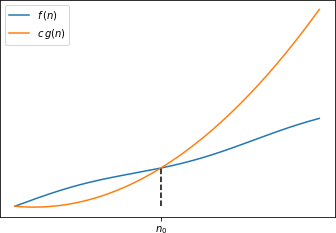
\includegraphics[scale=.8]{Imagenes/bigo.png}
    \caption{Representación de $f(n)= O(g(n))$}
    \label{fig:bigo}
\end{figure}

Se dice que un algoritmo es $O(g(n))$ si el número de operaciones que requiere para resolver un problema de tamaño $n$ es $O(g(n))$.
%
Por ejemplo, el algoritmo para sumar dos números de $n$ dígitos toma $O(n)$ operaciones (al considerar que nuestra operación básica es sumar dígitos).

\subsection*{Clases \textbf{P}, \textbf{NP} }
Un algoritmo para resolver algún problema puede tener como resultado cualquier cosa; por ejemplo un número si el problema es una suma, un polígono si buscamos una envolvente convexa, una función si resolvemos una ecuación diferencial o hasta una palabra como \texttt{sí} o \texttt{no} si buscamos saber si un número es primo.
%
Este último tipo de problema es un ejemplo de una clase importante llamada problemas de decisión. Estos problemas son de interés teórico en la teoría de la complejidad por tener una salida muy simple y porque una gran cantidad de otro tipo de problemas pueden formularse como problemas de decisión. 
%
Las clases de complejidad más analizadas están definidas para estos problemas de decisión.

%TODO: hablar de problemas de decisión
Dos de las clases más analizadas son las siguientes:

\begin{itemize} 
    \item \textbf{P}. Engloba a los problemas para los que existe un algoritmo que los resuelve y que toma a lo más $Kn^c$ operaciones con $K,c$ finitas. 
		%
		El nombre de esta clase hace referencia a que pueden resolverse en tiempo polinomial es decir que toman $O(n^c)$ operaciones para alguna $c$ positiva y finita. 

    \item \textbf{NP}. Engloba a los problemas para los que se puede verificar que se encontró una solución en tiempo polinomial. \footnote{Una definición alternativa pero equivalente se basa en el concepto de máquinas de turing no deterministas.}
\end{itemize}

Una subclase importante de la clase \textbf{NP} es la llamada \textbf{NP-completo} que incluye a los problemas para los cuales hallar un algoritmo de solución 
en tiempo polinomial implica hallar uno para todos los problemas en \textbf{NP}. 
%
De modo intuitivo es el conjunto de los problemas más difíciles en la clase.

Claramente \textbf{P} $\subseteq$ \textbf{NP}\footnote{Si ya tenemos un algoritmo que resuelve un problema en tiempo polinomial, para verificar si una solución es correcta 
solo hay que resolver el problema} pero determinar si también se cumple esta relación en sentido contrario, es decir, determinar si \textbf{P} = \textbf{NP}, es un problema 
sumamente difícil con implicaciones importantes que no ha sido resuelto.

La distinción en algoritmos que toman tiempo polinomial podría parecer arbitraria.
%
Sin embargo, es importante porque los polinomios ejemplifican funciones de crecimiento lento y cumplen con varias propiedades teóricas que simplifican la clasificación 
de los problemas~\cite{wigderson2006p}.

%TODO: pasan a NP-hard, distinguir el JSP como NP-Completo, es decir, como problema de decisión, y el problema de optimización asociado, que es NP-hard.
%Creo que lo mejor es crear una subseción {Clase NP-hard}


\subsubsection*{Clase NP-hard}
Las clases de complejidad antes mencionadas se definieron para problemas de decisión pero son útiles para clasificar otros tipos de problemas. En particular la clase \textbf{NP-hard} sirve para clasificar problemas de optimización como el JSP . \\
Se dice que un problema de optimización pertenece a \textbf{NP-hard} si todos los problemas en \textbf{NP} pueden reducirse a él en tiempo polinomial. Para los problemas de optimización que pertenecen a esta clase no existe un algoritmo que encuentre la solución óptima en tiempo polinomial a menos que \textbf{P} = \textbf{NP}.  Es importante mencionar que el problema en cuestión no tiene por qué pertenecer a \textbf{NP}.

Muchos problemas de optimización de gran interés pertenecen a la clase \textbf{NP-hard}, entre ellos el JSP. Cabe mencionar que al JSP se le puede asociar un problema de decisión que consiste en determinar si una solución dada es óptima o no siendo este problema \textbf{NP-completo}. 
%
Ante la dificultad para resolver estos problemas de manera eficiente surgieron técnicas conocidas como metaheurísticas que buscan facilitar encontrar soluciones aceptables aunque no óptimas.


